\section{The Hybrid Agentic Framework}
\label{sec:framework}


In this section, we present the design of our LLM-based solver. The core philosophy of our framework is the strict separation of concerns: rather than employing a single ``black box'' model, we architect a modular system where specialized agents handle distinct cognitive tasks: ambiguity resolution, mathematical optimization, and semantic interpretation.

This design enables us to bridge the gap between the ambiguous descriptions often found in real-world business and the precise inputs required by formal inventory models (formulated in \Cref{sec:InventoryModel}). By organizing these agents into a collaborative workflow, our system functions as a ``cognitive scaffold'': it standardizes human inputs for rigorous solving and subsequently interprets the mathematical results into actionable insights.

We begin by describing the structure of the agentic pipeline, followed by a detailed breakdown of each individual agent.


\vspace{-.5em}

\subsection{Pipeline Architecture}

Our framework integrates human-like problem input, structured information extraction, adaptive optimization, and verbal policy interpretation into a coherent pipeline (\Cref{fig:pipeline}).
	The pipeline is composed of three interconnected components that together transform informal descriptions into optimized inventory policies. % \vspace{-.3em}
    \begin{figure}[!t]
		\centering
        \vspace{-.5em}
		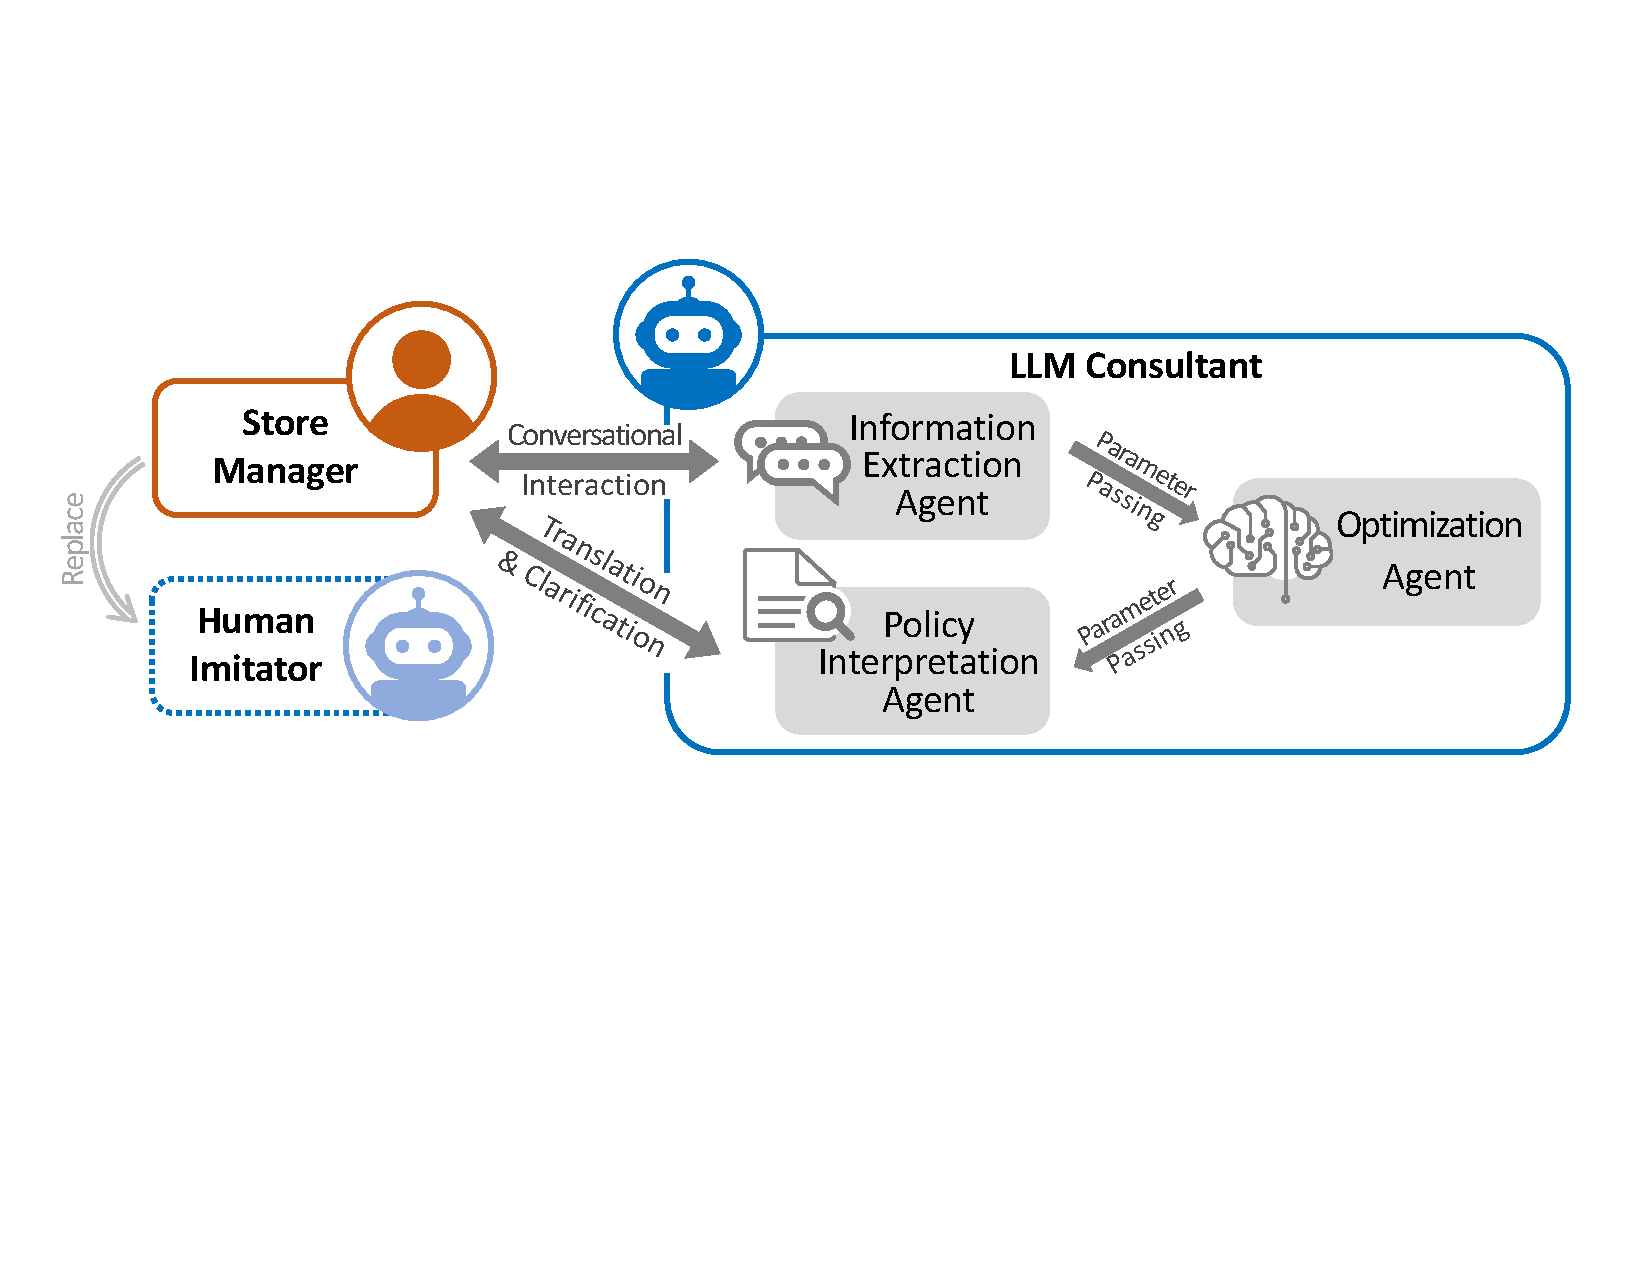
\includegraphics[width = \linewidth]{fig/teaser_new.pdf} % \vspace{-.5em}
		\caption{LLM-Agent Pipeline for Inventory Management}
		\label{fig:pipeline}
        % \vspace{-1em}
	\end{figure}
    \begin{description}[leftmargin=4em, labelsep=1em] % \itemsep = -.1em
		\item[Information Extraction Agent.] This agent converses with the human user, interprets the user's informal input, and incrementally converts it into structured parameters. Through conversational rounds, it asks clarifying questions, fills missing entries, and resolves conflicts until a complete and consistent parameter table is obtained.
		\item[Optimization Agent.] Once the problem is fully specified, the Optimization Agent invokes appropriate solvers, such as those for the classical $(s, S)$ policy and deep reinforcement learning algorithms, to generate inventory policies. The choice of the recommended policy depends on user-defined preferences, e.g., trading off expected cost against cost variance.
        \item[Policy Interpretation Agent.] Once the Optimization Agent identifies a recommended policy, this policy is passed to the Policy Interpretation Agent, which intuitively explains the nature of the policy to the user, responds to optimal order quantity queries, and addresses any clarification questions.
		\end{description}
	Together, these components establish an iterative, human-like workflow that mimics real managerial practice while remaining fully automatable.



    
    
    \subsection{Information Extraction: Turning Dialogue into Parameters}


    

    When a user approaches our system for help with an inventory problem, the primary barrier to applying operations research methods is not optimization itself, but \emph{problem specification}: converting an informal, natural-language business description into a fully specified mathematical model. In our setting, the necessary information is provided incrementally through a multi-turn conversation, so the system must continuously extract, reconcile, and refine model parameters as the dialogue evolves. We assign this responsibility to the \textbf{Information Extraction Agent} (built on \emph{GPT-5-mini}\footnote{Unless otherwise noted, \emph{GPT-4o} serves as the baseline LLM throughout this paper. \emph{GPT-5-mini} is a smaller and weaker model; we use it here to reduce cost, as its performance is sufficient for the information-extraction task.}).

    In such conversational AI systems, relying solely on the model’s implicit memory---that is, the context window---is brittle for operations research applications. Long, unstructured dialogues are prone to \emph{context drift}, in which previously specified constraints are forgotten, and \emph{hallucination}, in which missing parameters are spuriously fabricated. To mitigate these failure modes, we adopt an \emph{Explicit Memory} architecture. Concretely, the agent is required to maintain a persistent \emph{Parameter Specification Table} (e.g., \Cref{tab:initial_params}) that represents the system’s authoritative epistemic state.
    
    The agent’s objective is then to populate this table by systematically eliciting, inferring, and validating all decision-relevant primitives. Through this process, the agent transforms an initially empty template (e.g., \Cref{tab:initial_params}) into a fully instantiated problem representation (e.g., \Cref{tab:completed_params}) that can be passed directly to the solver.
    
    
    \begin{table}[!ht]
        \centering
        \renewcommand{\arraystretch}{1.1}
        \begin{tabular}{P V U T}
            \toprule
            \textbf{Parameter} & \textbf{Value} & \textbf{Unit} & \textbf{Status} \\
            \midrule
            time\_horizon            & -- & --  & undefined \\
            demand\_type             & -- & N/A & undefined \\
            demand\_distribution     & -- & N/A & undefined \\
            perishability            & -- & N/A & undefined \\
            state\_transition\_model & -- & N/A & undefined \\
            holding\_cost            & -- & --  & undefined \\
            penalty\_cost            & -- & --  & undefined \\
            setup\_cost              & -- & --  & undefined \\
            lead\_time               & -- & --  & undefined \\
            max\_inventory           & -- & N/A & undefined \\
            max\_order               & -- & N/A & undefined \\
            risk\_tolerance          & -- & N/A & undefined \\
            \bottomrule
        \end{tabular}
        \caption{\textbf{Initial Parameter Specification for the Information Extraction Agent}}
        \vspace{1.2em}
        \label{tab:initial_params}
        
        \renewcommand{\arraystretch}{1.1}
        \begin{tabular}{P V U T}
            \toprule
            \textbf{Parameter} & \textbf{Value} & \textbf{Unit} & \textbf{Status} \\
            \midrule
            time\_horizon            & 60 & days & defined \\
            demand\_type             & random & N/A & defined \\
            demand\_distribution     & Poisson($\lambda=10$) & N/A & defined \\
            perishability            & TRUE & N/A & defined \\
            state\_transition\_model & lost\_sale & N/A & defined \\
            holding\_cost            & 5 & USD/unit/day & defined \\
            penalty\_cost            & 15 & USD/unit & defined \\
            setup\_cost              & 100 & USD/order & defined \\
            lead\_time               & 5 & days & defined \\
            max\_inventory           & 100 & N/A & defined \\
            max\_order               & 20 & N/A & defined \\
            risk\_tolerance          & 3 & N/A & defined \\
            \bottomrule
        \end{tabular}
        \caption{\textbf{Example of a Completed Parameter Specification}}
        \label{tab:completed_params}
    \end{table}

    \begin{figure}[!t]
		\centering
        \vspace{-.5em}
		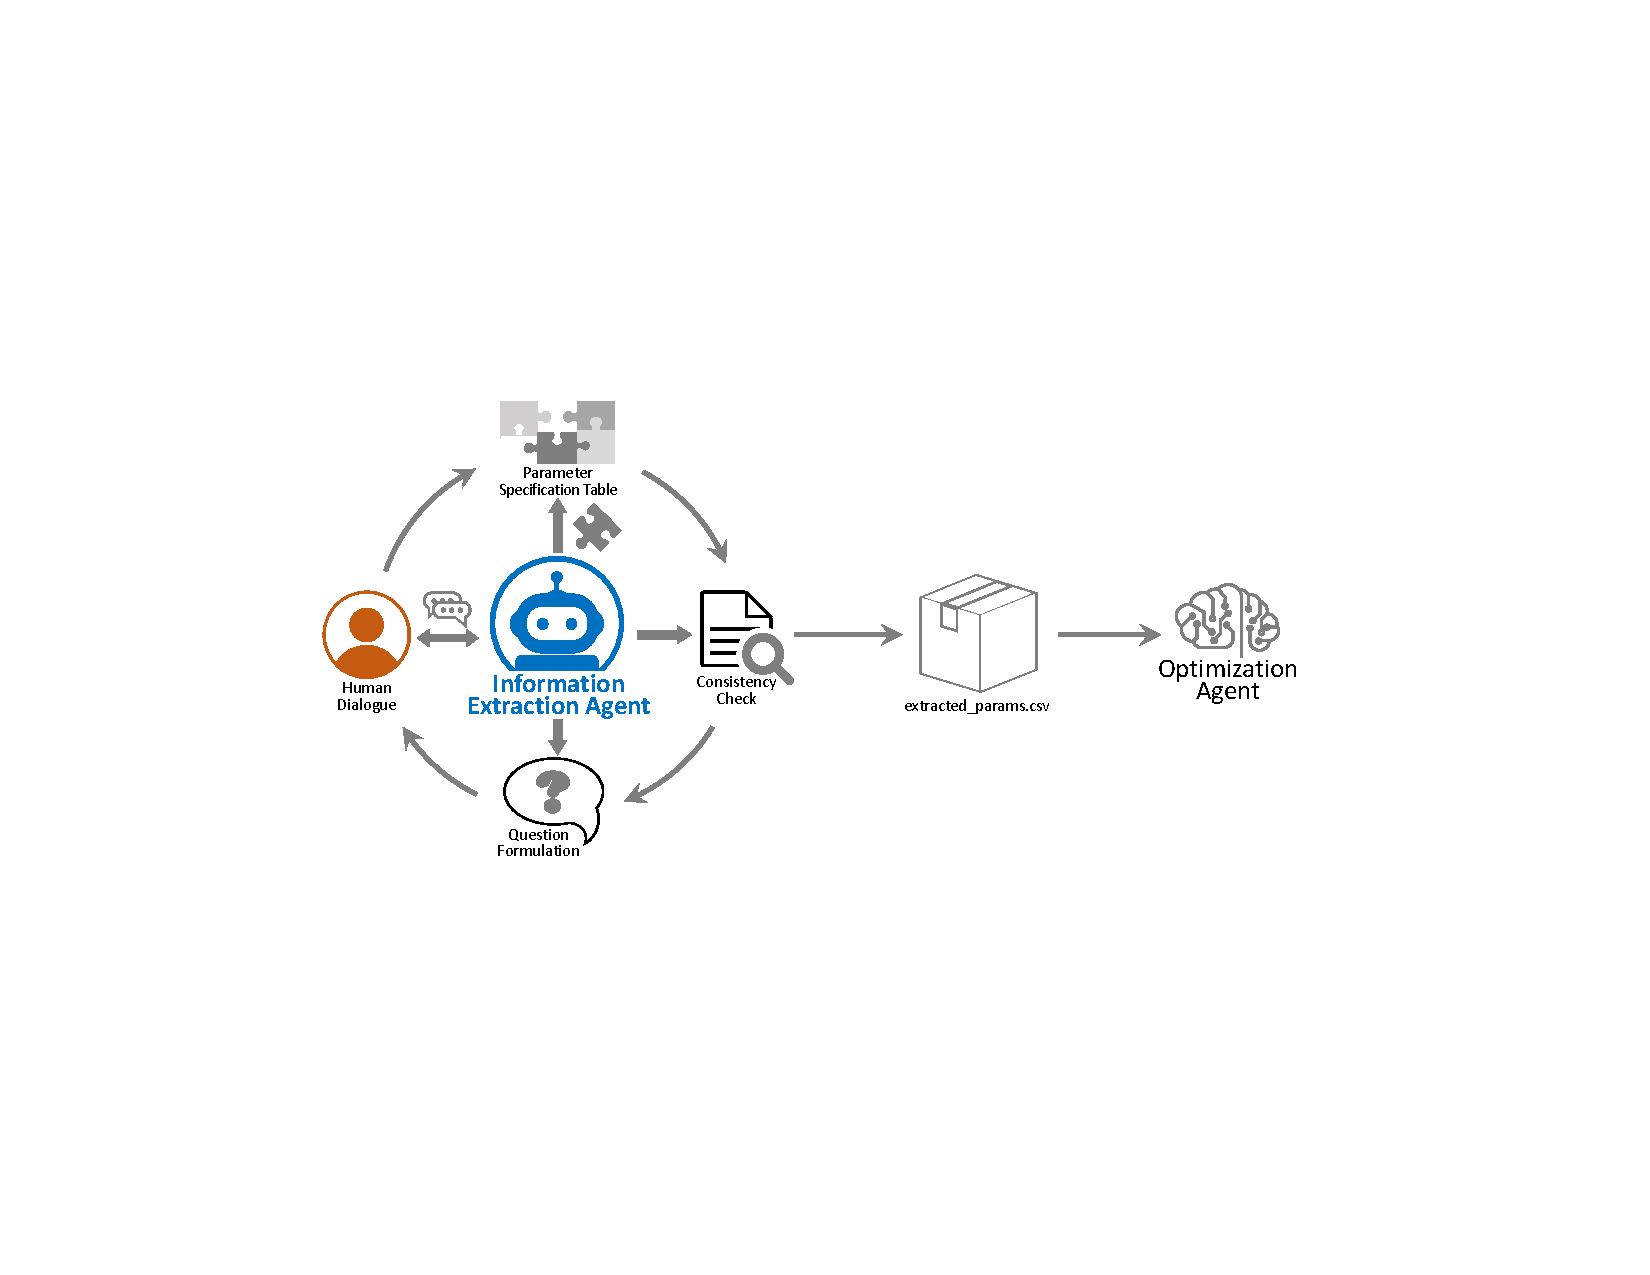
\includegraphics[width = 0.8\linewidth]{fig/Information_Extraction_Agent.pdf} % \vspace{-.5em}
		\caption{Architecture of the Information Extraction Agent}
		\label{fig:info_extra}
        % \vspace{-.5em}
	\end{figure}
    
    More concretely, the conversational process unfolds in rounds. In each round, the Information Extraction Agent analyzes the user's latest response and performs the following actions:
    \begin{enumerate}
        \item \emph{Update Table:} If new, credible information is identified, it fills the corresponding blank in the table and updates the status to ``defined.''
        \item \emph{Detect Conflicts:} If the user provides information that contradicts a previously defined entry, the agent flags the conflict for resolution.
        \item \emph{Formulate Question:} If the table contains undefined variables or identified conflicts, the agent generates a targeted question to clarify ambiguities or gather missing data. The conversation continues to the next round.
    \end{enumerate}
    The dialogue concludes when all parameters are marked as ``defined'' and the system verifies that no conflicts exist. A visual representation of this complete workflow is provided in \Cref{fig:info_extra}.
    For reproducibility, the exact system prompt used by the Information Extraction Agent is documented in \Cref{tab:system_prompt_info_extraction} (\Cref{sec:system_prompts}). Furthermore, we provide representative conversation logs in \Cref{sec:example1,sec:sample_conversation}; specifically, Examples 3--5 highlight the agent's capability to navigate ambiguity and resolve logical conflicts effectively.

    
    
    
    Upon successful termination, the Information Extraction Agent saves two files: 
    \begin{itemize} 
        \item \texttt{extracted\_params.csv}, containing the extracted parameters from the conversation; and 
        \item \texttt{conversation\_log.txt}, containing the complete conversation history. 
    \end{itemize}
    Finally, it invokes the Optimization Agent, which uses the \texttt{extracted\_params.csv} file to calculate and propose a recommended inventory policy.


\begin{remark}[Comparison with DPLM]
    With the above extraction-and-memory mechanism in place, we now situate our approach relative to recent efforts on automating operations-research modeling.
    We position our work by contrasting it with the recent Dynamic Programming Language Model (DPLM) proposed by \citet{zhou2025auto}. While sharing the ultimate goal of automating operations research modeling, our approaches differ fundamentally in their handling of information ambiguity and training methodology. \citet{zhou2025auto} demonstrate that a specialized fine-tuning pipeline trained on synthetic data can effectively translate fully specified, static textbook descriptions into mathematical models. In contrast, our framework addresses the \emph{preceding} challenge of real-world ambiguity, where problem definitions must be interactively elicited and maintained through unstructured dialogue. We demonstrate that for this extraction phase, rigorous prompt engineering with a capability-rich foundation model (\emph{GPT-5-mini}) and explicit memory management yields high-fidelity results without requiring the extensive supervised fine-tuning and reinforcement learning resources detailed in \citet{zhou2025auto}. However, their rigorous synthetic data generation (DualReflect) and fine-tuning recipes offer a valuable roadmap for future enhancements, particularly for distilling our extraction capabilities into smaller, more efficient models or for improving the system's ability to auto-formulate novel constraints that fall outside standard inventory templates.
\end{remark}
    
    

    
    

    \subsection{Optimization: From Parameters to Policies}



    With the problem structure specified, the \textbf{Optimization Agent} then executes the core algorithmic work. Unlike a generic LLM that might ``hallucinate'' a solution, this agent acts as a dispatcher for rigorous operations research solvers. The corresponding workflow is illustrated in Figure \ref{fig:LLM_Solver}.

    





    A key feature of our optimization module is the integration of user risk preferences. We recognize that normative optimality is not single-dimensional; users often trade off expected cost against stability. To capture this, the agent elicits a preference parameter $\lambda \in [-10, 10]$, which weights the penalty for variance (risk). The agent then selects the policy $\policy$ that minimizes the following composite objective:
    \begin{equation}\label{eqn:objective}
        \mathcal{L}(\policy) \; = \; \mathds{E}\big[\mathrm{Cost}(\policy)\big] \; + \; \exp(-\lambda) \, \cdot \, \mathrm{Std}\big[\mathrm{Cost}(\policy) \big] \, ,
    \end{equation}
    where $\mathrm{Cost}(\policy)$ represents the expected cost and $\mathrm{Std}(\policy)$ represents the cost standard deviation under policy $\policy$.



\begin{figure}[!t]
    \centering
    % \vspace{-.5em}
    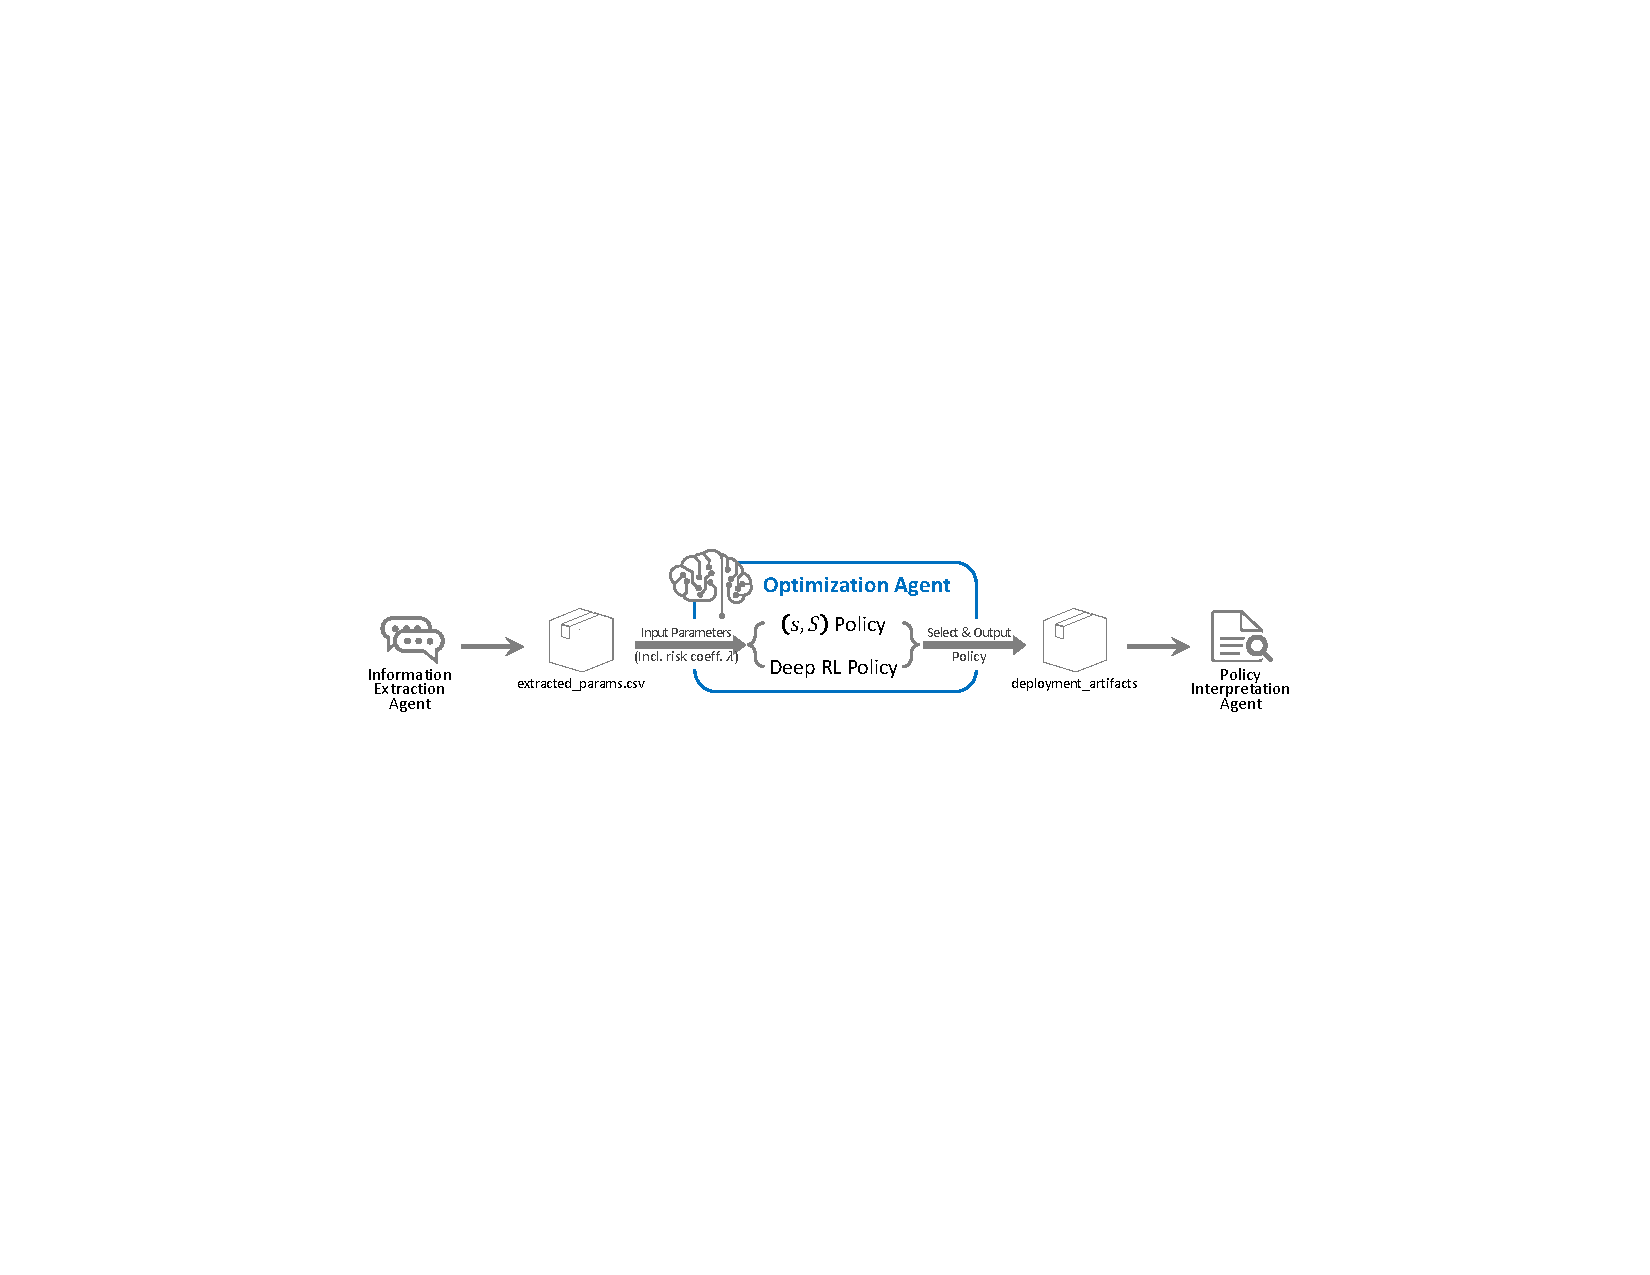
\includegraphics[width = \linewidth]{fig/optimizer_new.pdf} 
    \vspace{-2em}
    \caption{Architecture of the Optimization Agent}
    % \vspace{-.2em}
    \label{fig:LLM_Solver}
\end{figure}

In our current implementation, the agent arbitrates between two distinct policy classes, representing the spectrum from classical theory to modern AI:

\begin{description}
    \item[The $(s, S)$ Policy (Classical Heuristic):] The $(s, S)$ policy is a classic inventory management approach defined by a reorder point $s$ and an order-up-to level $S$. When the inventory level (the sum of on-hand inventory and orders in the pipeline) drops to or below $s$, a replenishment order is triggered to bring the stock back up to $S$. This policy effectively balances ordering and holding costs by maintaining inventory within these thresholds, ensuring stock is replenished only when necessary. It is particularly effective in systems with positive lead times. While the policy is simple to implement and interpret, improper values for $s$ and $S$ can lead to significant overstocking or stockouts. Our Optimization Agent simulates the expected cost and variance across a grid of $(s, S)$ parameter choices to identify the best $(s, S)$ configuration.
    \item[Deep Q-Network (Deep Reinforcement Learning):] The DQN policy is based on the Markov Decision Process~(MDP) formulation of the inventory problem (detailed in \Cref{sec:InventoryModel}). It is a reinforcement learning method that combines Q-learning with deep neural networks to learn optimal policies in dynamic environments. Rather than maintaining a Q-table, which is infeasible for large state-action spaces, DQN uses a neural network to approximate the Q-value function, predicting the expected cumulative reward for each action given a state. We define the state space as the composition of the current inventory position, the time period, and the vector of orders in the pipeline. By iteratively updating the Q-network via the Bellman equation, DQN approximates optimal policies using samples from the demand distribution. Notably, DQN performs well even when the lead time is large due to its ability to handle sequential decision making problems with high-dimensional input.    
    \end{description}    
    These two paradigms represent an inherent trade-off between \textit{expected efficiency} and \textit{operational stability}. While the Deep RL policy leverages high-dimensional feature extraction to aggressively minimize expected costs, its stochastic nature may introduce higher variance. Conversely, the $(s, S)$ heuristic, though potentially conservative, offers a robust and predictable baseline.   
    Our framework addresses this dichotomy through an \textit{agentic design}: the Optimization Agent interprets the user's risk tolerance and performs meta-reasoning to arbitrate between the solvers, selecting a policy that balances expected cost and operational stability.


    
        Upon convergence, the Optimization Agent serializes the model artifacts to a directory named \texttt{deployment\_artifacts}, containing three files:
    
    \begin{itemize}
        \item \texttt{config.json}: Includes important instance parameters (e.g., lead time, maximum inventory, time horizon, and the state and action dimensions of the DQN network).
        \item \texttt{dqn\_weights.pth}: Contains the weights of the DQN network.
        \item \texttt{policy\_evaluation\_results.csv}: Stores the average cost and standard deviation of the optimal DQN policy and $(s, S)$ policy, respectively, along with the optimal $s$ and $S$ values.
    \end{itemize}
    These artifacts serve as the essential input for the subsequent Policy Interpretation Agent.

\begin{remark}[Extensibility to Novel Algorithms]
    Although our experiments focus on $(s,S)$ and DQN policies, the modular architecture of the Optimization Agent facilitates the seamless integration of additional policy classes and emerging algorithms. Unlike black-box AI models, where enhancing algorithmic reasoning often necessitates resource-intensive retraining or fine-tuning, our framework treats solvers as interchangeable modules. This design allows researchers to effortlessly incorporate novel optimization techniques, thereby ensuring the system remains at the frontier of operations research without altering the core linguistic interface.
\end{remark}

    
    
    \subsection{Policy Interpretation: Communicating Policies in Words}
    The final component, the \textbf{Policy Interpretation Agent}, ingests the artifacts produced by the Optimization Agent and translates them into actionable business intelligence. This stage is critical for realizing actual cost reductions: theoretical optimality translates to practical efficiency only when human decision-makers trust and adhere to the algorithmic suggestions.\footnote{Pre-LLM studies of automated replenishment already document that store managers frequently deviate from optimization-based order recommendations and that accounting for their behavioral responses is essential for effective system design \citep{van2010ordering}.} 
    To mitigate algorithm aversion and foster cognitive alignment, this agent navigates the trade-off between \emph{performance} (lower cost $\mathcal{L}(\policy)$ in \cref{eqn:objective}) and \emph{interpretability}.

    Because the $(s, S)$ policy is generally more interpretable and familiar to practitioners, while the DQN policy is less transparent but typically achieves lower costs, the Decision Interpretation Agent follows the communication protocol below:

    \begin{description}
        \item[\textbf{Scenario A:} The $(s, S)$ Policy Performs Better.] 
If the $(s, S)$ heuristic yields a lower objective value $\mathcal{L}(\policy)$, the agent leverages its inherent interpretability. It provides a detailed yet accessible explanation of the reorder point $s$ and order-up-to level~$S$, describing how the policy operates in day-to-day inventory decisions. It then invites the user to ask follow-up questions or relate the thresholds to their own operational experience.

        
    
        \item[\textbf{Scenario B:} The DQN Policy Performs Better.] If the DQN policy yields a lower objective value~$\mathcal{L}(\policy)$, the agent first offers a high-level overview of the black-box policy, framing it as an ``on-demand expert’’: at any time step, given the current inventory position and pipeline orders, the user can query the agent for a recommended order quantity. If the user finds this lack of interpretability unsatisfying and prefers a more intuitive explanation, the agent then additionally presents the suboptimal $(s, S)$ policy, reports the percentage difference in the optimization objective between the two policies (e.g., ``If you're interested in a simpler policy, the $(s=2, S=11)$ policy exists but it costs 20.5\% more''), and allows the user to decide which policy they ultimately wish to adopt.
        
    \end{description}

    Throughout this interaction, the agent remains responsive to user inquiries, clarifying the rationale behind specific recommendations to reinforce trust. Once the user indicates understanding or signals readiness to adopt the policy, the agent terminates the conversation and archives the dialogue transcript as \texttt{interpret.txt} for audit and analysis. An illustrative example of this interaction is provided in \Cref{fig:interpretation}.

    \begin{figure}[!t]
    \centering
    % \vspace{-.5em}
    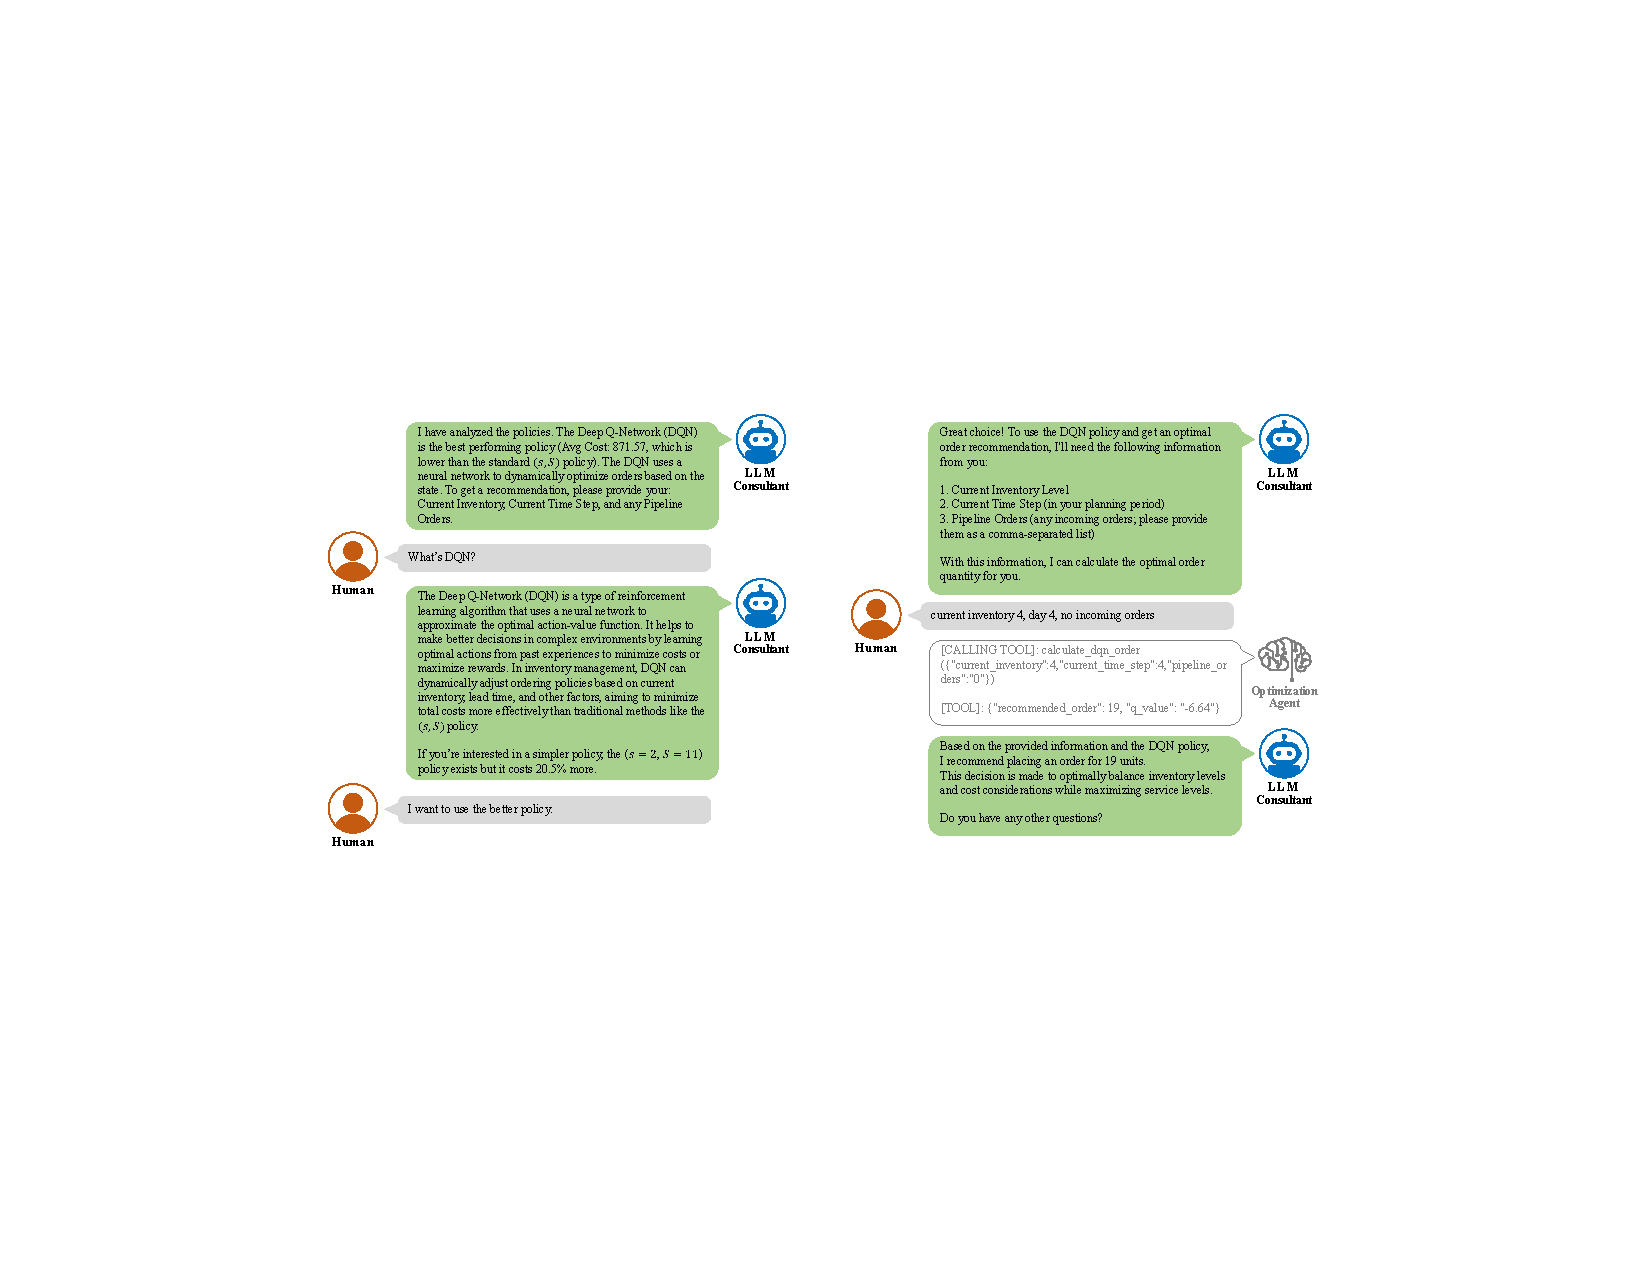
\includegraphics[width = \linewidth]{fig/interpretation2.pdf} 
    \vspace{-2em}
    \caption{Representative dialogue between the Human User and the Policy Interpretation Agent.}
    % \vspace{-.2em}
    \label{fig:interpretation}
\end{figure}




